
\documentclass[11pt]{article}

\usepackage{amsmath,amssymb}
\usepackage{booktabs}
\usepackage{graphicx}
\usepackage[hyphens]{url}
\usepackage{hyperref}
\usepackage[margin=1in]{geometry}
\usepackage[round,authoryear]{natbib}
\usepackage{xcolor}
\usepackage{array}
\usepackage{enumitem}
\usepackage[affil-it]{authblk}
\usepackage{tikz}
\usetikzlibrary{decorations.pathreplacing}

\renewcommand{\arraystretch}{1.3}

\newcommand{\todo}[1]{\textcolor{red}{[TODO: #1]}}
\newcommand{\pending}{\textcolor{orange}{\emph{pending}}}

\title{Two of Ten Nucleotide Foundation Models Encode Base-Pairing\\
Partners After Composition Control}

\author{Elliot Tower}
\affil{Independent researcher \\ \texttt{elliot@elliottower.ai}}
\date{}

\begin{document}
\maketitle

\begin{abstract}
\noindent\textbf{Motivation:}
RNA foundation models appear to encode secondary structure, but stems
are GC-rich and loops are AU-rich, so any composition-sensitive
embedding inherits this correlation as apparent structure awareness.
Existing benchmarks do not control for this confound.

\noindent\textbf{Results:}
We evaluate ten models across 52 Rfam families using a three-rung
ladder that progressively strips composition shortcuts. After
nucleotide-stratified and dinucleotide null controls, eight of ten
models retain signal in at most two families. Only ERNIE-RNA and
RiNALMo pass all three rungs, including partner specificity---knowing
which position pairs with which (PS~$= 0.120$ and $0.215$,
precision~$> 87\%$). The remaining eight fall two or more orders of
magnitude below, with Caduceus the only one exceeding the 1/3
partner-is-max baseline. Transversion controls on all ten models confirm
the methodology measures structural sensitivity rather than
Watson-Crick complement logic. A synthetic covariation control places
an upper bound of $\sim$30\% on the contribution of learned geometric
sensitivity beyond sequence covariation. The confirmatory hypotheses are
preregistered; controls added during revision are identified as post hoc.

\noindent\textbf{Availability:}
Code, data, and preregistration documents at
\url{https://github.com/elliottower/rna-structure-awareness}; Zenodo
DOI: 10.5281/zenodo.21362717. CC-BY-4.0.
\end{abstract}


%% ======================================================================
\section{Introduction}
%% ======================================================================

Foundation models pretrained on nucleotide sequences are increasingly
used for RNA secondary structure prediction, drug target
identification, and splice-site recognition. A basic question
underlies all of these applications: do these models actually
encode base-pairing structure---the pattern of intramolecular
Watson-Crick pairing that governs RNA stability and function---or
are their representations picking up on something simpler?

The answer turns out to be ``something simpler,'' at least for most
models. RNA secondary structure introduces a systematic composition
confound. Stems are GC-rich (68.5\% GC) because Watson-Crick pairing
favors G-C and C-G. Loops are AU-rich (43.9\% GC) because unpaired
regions tolerate all four nucleotides more equally. Any embedding
metric sensitive to nucleotide identity inherits this 24.7
percentage-point enrichment as an apparent structure signal. We
initially used Grassmannian geodesic distance to compare embedding
subspaces between stems and loops, and found that a zero-parameter
3-mer frequency baseline matched trained models' scores. The models
were recognizing nucleotide composition, not structure.

This failure motivated a graded evaluation. The core idea is that
``structure awareness'' is not binary---it encompasses at least three
levels of resolution, each demanding strictly stronger knowledge:

\begin{enumerate}[nosep]
\item \textbf{Stem-vs-loop discrimination.} Can the model tell paired
  from unpaired positions? Any representation sensitive to nucleotide
  composition can do this, because stems and loops have different
  base frequencies.
\item \textbf{Discrimination surviving composition controls.} Does the
  signal persist after matching nucleotide and dinucleotide
  frequencies between stems and loops? This eliminates the dominant
  confound.
\item \textbf{Partner specificity.} Does the model know which
  \emph{specific} position pairs with which? If you mutate one base
  of a pair, does the model perturb the paired partner more than
  adjacent stem positions?
\end{enumerate}

\begin{figure}[htbp]
\centering
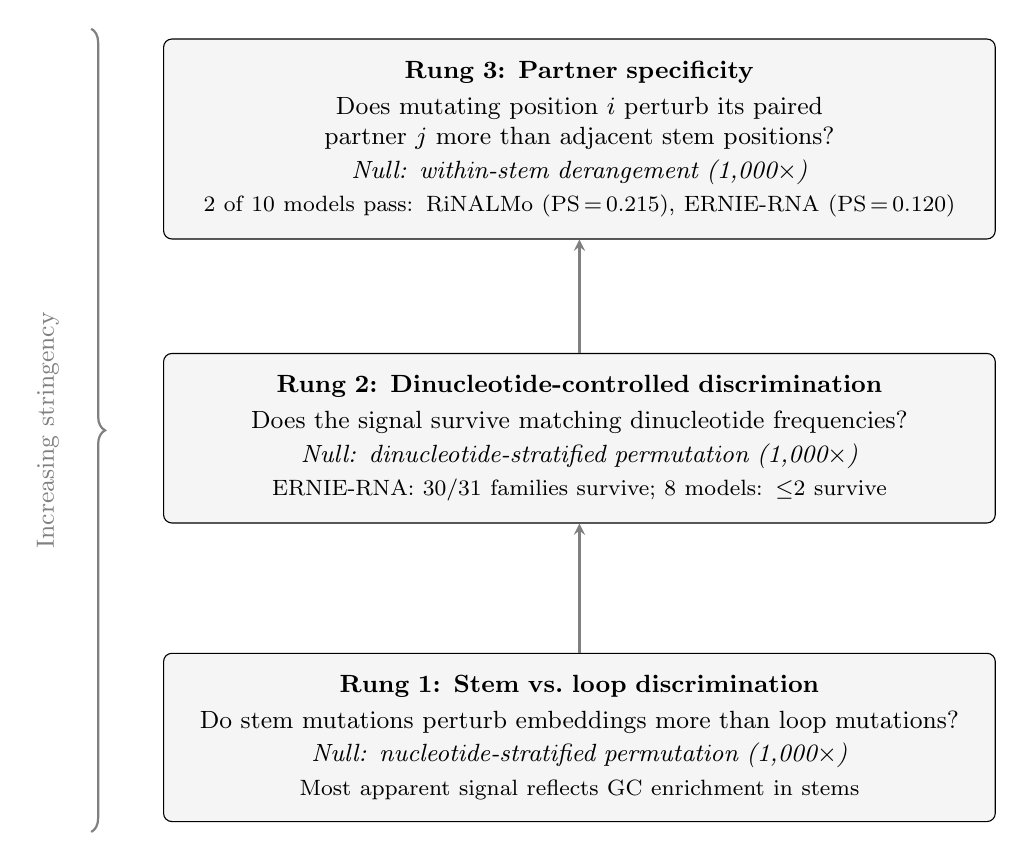
\begin{tikzpicture}[
  box/.style={draw, rounded corners=3pt, minimum width=10.5cm,
    text width=10cm, align=center, font=\small, inner sep=8pt},
  arr/.style={-stealth, thick, gray}
]
\node[box, fill=gray!8] (r1) at (0,0) {
  \textbf{Rung 1: Stem vs.\ loop discrimination}\\[2pt]
  Do stem mutations perturb embeddings more than loop mutations?\\[1pt]
  {\itshape Null: nucleotide-stratified permutation (1,000$\times$)}\\[1pt]
  {\footnotesize Most apparent signal reflects GC enrichment in stems}
};
\node[box, fill=gray!8] (r2) at (0,3.8) {
  \textbf{Rung 2: Dinucleotide-controlled discrimination}\\[2pt]
  Does the signal survive matching dinucleotide frequencies?\\[1pt]
  {\itshape Null: dinucleotide-stratified permutation (1,000$\times$)}\\[1pt]
  {\footnotesize ERNIE-RNA: 30/31 families survive; 8 models: $\leq$2 survive}
};
\node[box, fill=gray!8] (r3) at (0,7.6) {
  \textbf{Rung 3: Partner specificity}\\[2pt]
  Does mutating position $i$ perturb its paired partner $j$
  more than adjacent stem positions?\\[1pt]
  {\itshape Null: within-stem derangement (1,000$\times$)}\\[1pt]
  {\footnotesize 2 of 10 models pass: RiNALMo (PS\,=\,0.215),
  ERNIE-RNA (PS\,=\,0.120)}
};
\draw[arr] (r1.north) -- (r2.south);
\draw[arr] (r2.north) -- (r3.south);
\draw[decorate, decoration={brace, amplitude=5pt, mirror},
  thick, gray]
  (-6.2, -1.2) -- (-6.2, 9)
  node[midway, left=8pt, rotate=90, anchor=south, font=\small]
  {Increasing stringency};
\end{tikzpicture}
\caption{Three-rung evaluation ladder. Each rung applies a stricter
null model to separate genuine structure awareness from composition
artifacts. Permutation nulls at Rungs~1--2 control for nucleotide
and dinucleotide composition; the derangement null at Rung~3 tests
whether models encode specific pairing relationships.}
\label{fig:ladder}
\end{figure}

Existing evaluations of RNA foundation models typically assess
downstream task performance---secondary structure prediction
accuracy, splice-site classification, or contact-map
reconstruction---which conflate the model's structural knowledge
with the capacity of a fine-tuned head. Probing classifiers
\citep[e.g.,][]{rinalmo2025} test whether structural labels are
linearly decodable from representations, but remain susceptible to
the composition confound above. Our evaluation differs in two
respects: it uses composition-controlled nulls to separate genuine
structure signal from composition artifacts, and it tests causal
partner specificity through perturbation rather than correlation.

We apply this three-rung ladder (Figure~\ref{fig:ladder}) to ten
models across 52 Rfam families~\citep{rfam2021}. The
evaluation reveals a surprising asymmetry: the hardest test produces
the clearest positive result.


%% ======================================================================
\section{Models}
%% ======================================================================

\begin{table}[htbp]
\centering
\caption{Foundation model panel. Five RNA-pretrained, five
DNA-pretrained. Parameter counts span three orders of magnitude.}
\label{tab:models}
\small
\begin{tabular}{llrll}
\toprule
\textbf{Model} & \textbf{Architecture} & \textbf{Params} & \textbf{Tokenization} & \textbf{Domain} \\
\midrule
RNA-FM~\citep{rnafm2022}         & BERT encoder       & 99M  & Character   & RNA \\
ERNIE-RNA~\citep{ernierna2025}   & BERT encoder       & 86M  & Character   & RNA \\
RiNALMo~\citep{rinalmo2025}     & Encoder            & 650M & Character   & RNA \\
UTR-LM~\citep{utrlm2024}        & BERT encoder       & $\sim$2M & Character & RNA (5$'$ UTR) \\
SpliceBERT~\citep{splicebert2024} & BERT encoder     & 19M  & Character   & RNA (pre-mRNA) \\
NT~v2~\citep{ntv22024}           & ESM + GLU          & 56M  & 6-mer       & DNA \\
DNABERT-2~\citep{dnabert22024}   & MosaicBERT         & 117M & BPE         & DNA \\
HyenaDNA~\citep{hyenadna2023}   & Hyena SSM          & 5.4M & Character   & DNA \\
Caduceus~\citep{caduceus2024}    & BiMamba SSM        & 14M  & Character   & DNA \\
Evo~\citep{evo2024}              & StripedHyena       & 7B   & Byte-level  & DNA \\
\bottomrule
\end{tabular}
\end{table}

Architectures include attention-based encoders (RNA-FM, ERNIE-RNA,
RiNALMo, UTR-LM, SpliceBERT, NT~v2, DNABERT-2), state-space models
(HyenaDNA, Caduceus), and a hybrid (Evo). Tokenization strategies
include character-level, 6-mer, byte-pair encoding, and byte-level.

The panel was selected to cover the major architectural families
(encoder, SSM, hybrid), tokenization strategies, pretraining domains
(RNA vs DNA), and parameter scales (2M--7B) among publicly available
models with released weights. Models without public weights or
without single-sequence inference capability at the time of evaluation
(such as RNA-MSM, Uni-RNA, and AIDO.RNA) were excluded. The framework
is designed to accommodate additional models as they become available.


%% ======================================================================
\section{Methods}
%% ======================================================================

\subsection{RNA structure dataset}

52 RNA families drawn from Rfam~14.10~\citep{rfam2021}, spanning
tRNAs (7 families), rRNAs (4), ribozymes (6), riboswitches (8),
snRNAs (5), cis-regulatory elements (9), miRNA precursors (5),
CRISPR repeats (3), and other ncRNAs (5).
Sequence lengths range from 22 to 301~nt (median 89~nt, IQR 56--132).
This sample covers $<$2\% of the $>$4{,}000 Rfam families but
spans the major structural classes of well-characterized ncRNAs.
Long-range pairing ($>$150~nt), multi-domain ribozymes, and
thermoswitches are underrepresented; extending the evaluation to
larger, more complex structures is a priority for future work.
Three families were excluded post hoc for unbalanced dot-bracket
annotations (ambiguous stem/loop assignments), leaving 49 evaluable
families for Rungs~1--2.

One representative sequence per family is drawn from the Rfam seed
alignment, selected as the seed sequence with highest bit score.
This single-sequence design trades within-family coverage for breadth;
Section~\ref{sec:limitations} quantifies this tradeoff. Each
family has an experimentally supported secondary structure from Rfam
consensus or PDB crystal structure.
Preregistration documents (Phase~1 SHA \texttt{694b43b}, Phase~2
\texttt{bd4b3fd}, Phase~6 \texttt{c19aa59}) are deposited with the
code.
Positions are labeled stem
(base-paired) or loop (unpaired) from dot-bracket annotation.
Minimum criteria: $\geq 20$~nt, $\geq 5$ stem and 5 loop
positions. For the
partner-specificity rung, families require $\geq 15$ Watson-Crick
pairs with $\geq 3$ eligible pairs per stem ($K \geq 3$) to support
the derangement null; 34 families qualify (18 excluded by pair count,
3 by the annotation filter above).

\subsection{Rung 1: Do stems respond differently than loops?}

The idea is simple: mutate a position to its Watson-Crick complement
(A$\leftrightarrow$U, C$\leftrightarrow$G) and measure how much the
model's embedding changes. If the model encodes structure, stem
positions should respond more strongly than loop positions, because
mutations in stems disrupt a pairing relationship. The structure
sensitivity ratio is:

\begin{equation}
R = \max_{\ell} \frac{\bar{d}_{\text{stem}}^{(\ell)}}{\bar{d}_{\text{loop}}^{(\ell)}}
\end{equation}

The catch is that this ratio will be inflated even without any
structural knowledge, because stems and loops have different
nucleotide frequencies. A model that simply responds differently to
G$\to$C mutations than to A$\to$U mutations will show apparent
structure sensitivity.

\paragraph{Composition null.}
To control for this, we shuffle stem/loop labels independently within
each nucleotide type (A, U, G, C). This preserves per-nucleotide
composition while destroying the structure-label association. For each
of 1,000 permutations, we compute $R$ at every layer and take the
maximum. The 95th percentile of these 1,000 max-over-layers values
sets the null threshold. Any model exceeding this threshold shows
genuine structure sensitivity beyond composition.

\paragraph{Untrained baseline.}
RNA-FM with randomized weights serves as the composition-only control.

\subsection{Rung 2: Does the signal survive dinucleotide controls?}

The first-order null controls for single-nucleotide composition, but
stems and loops also differ in dinucleotide context (stem-G usually
occurs in GC pairs; loop-G occurs in diverse contexts). The
dinucleotide null shuffles labels within each dinucleotide type
(previous + current nucleotide: AA, AC, AG, \ldots), providing a
stricter control. Families exceeding the first-order null are tested
against this second-order control.

\subsection{Attention-contact correlation}
\label{sec:methods-attn}

For models with accessible attention matrices, we compute Spearman
rank correlation between symmetrized attention weights and a binary
contact matrix (1 for base-paired positions, 0 otherwise). For
NT~v2's 6-mer and DNABERT-2's BPE tokenization, contacts are
aggregated to the token level.

All attention-contact correlations use eager attention computation
(\texttt{attn\_implementation="eager"}).
HuggingFace Transformers' default SDPA backend can silently return
\texttt{None} for attention weights when
\texttt{output\_attentions=True}; downstream code that interprets
absent attention as zero correlation produces spurious results.
Library versions and a detailed disclosure are documented in the
code repository.

For DNABERT-2, MosaicBERT's fused Wqkv projection and ALiBi
position biases prevent standard attention extraction. We compute
content-only attention by hooking the Wqkv output, splitting into Q
and K, and computing
$\mathrm{softmax}(QK^T / \sqrt{d_k})$ without ALiBi. The resulting
correlation reflects learned query-key patterns; the full model's
attention is dominated by local position bias, so the
content-only value is an upper bound on the structure signal at
inference.

To distinguish learned from architectural attention, we evaluate
each model with both trained and randomly initialized weights
(Table~\ref{tab:attn_trained_untrained}).

\subsection{Structure probing}

Per-position hidden-state vectors are extracted from each layer (or
equivalent hidden state for SSMs). Logistic regression on these
vectors predicts stem vs loop, using GroupKFold cross-validation by
RNA family to test cross-family generalization. The best layer is
selected by maximum balanced accuracy across all layers. Probing
$\Delta$ is balanced accuracy minus 0.5 (the chance level for
balanced accuracy), reported at the best layer.

\subsection{Rung 3: Does the model know which position pairs with which?}

This is the hardest test. The intuition: if you mutate one base in a
pair, a model that truly understands pairing should perturb the
partner's embedding more than adjacent stem positions. Knowing that
``this is a stem'' is Rung~1. Knowing that ``position 15 pairs with
position 42'' is Rung~3.

For each Watson-Crick base pair $(i, j)$ in a stem with $\geq 3$
eligible pairs:

\begin{enumerate}
\item Mutate position $i$ to its Watson-Crick complement.
\item Measure the cosine distance between wild-type and mutant
  embeddings at every other stem position.
\item Compute perturbation specificity:
  $\text{PS}(i, j) = \Delta_j - \max(\Delta_{j-1}, \Delta_{j+1})$,
  where $\Delta_j$ is the cosine distance at the paired partner and
  $\Delta_{j \pm 1}$ are distances at adjacent stem positions.
\end{enumerate}

A positive PS means the model perturbs the correct partner more than
its neighbors---it knows who pairs with whom.

\paragraph{Positive control gate.}
Each family must show significantly greater stem perturbation than
loop perturbation (paired $t$-test, $p < 0.05$). Families failing
this gate are excluded.

\paragraph{Derangement null.}
For each stem with $K \geq 3$ eligible pairs, 1,000 derangements
permute partner labels within the stem. The real PS is compared
against the distribution of deranged PS values. A family exceeds the
null if the observed mean PS exceeds the 95th percentile.

\paragraph{Partner-is-max (H3).}
For deep-interior pairs, the fraction where the true partner receives
the maximum perturbation among all stem positions. Chance baseline is
$1/3$; preregistered threshold is binomial $> 1/3$.

\subsection{Preregistered hypotheses}

\textbf{Phases 1--2} (composition-controlled discrimination):
\begin{itemize}[nosep]
\item H1: RNA-FM trained/untrained ratio $\geq 2.0$
\item H6: RNA-FM ratio $\geq 2.0$ at $N = 52$ (powered replication)
\item H7: $\geq 1$ family exceeds dinucleotide null
\item H10: RNA-FM trained $>$ untrained in $\geq 75$\% of families
\item H11: NT~v2 attention $\rho > 0.15$ trained AND $< 0.05$ untrained
\end{itemize}

\textbf{Phase 6} (partner specificity, Bonferroni $\alpha = 0.05/3 = 0.0167$):
\begin{itemize}[nosep]
\item H1$_6$: At least one model has mean PS $> 0$ with $\geq 7$
  families exceeding derangement null (Wilcoxon)
\item H2$_6$: RNA-pretrained models have higher PS than DNA-pretrained
  models (rank-biserial $> 0.5$)
\item H3$_6$: At least one model has partner-is-max fraction exceeding
  $1/3$ (binomial)
\end{itemize}


%% ======================================================================
\section{Results}
%% ======================================================================

\subsection{Rung 1: Composition absorbs most of the signal}

Once the composition null is applied, most models' apparent structure
sensitivity shrinks dramatically. RNA-FM's signal drops from
$\sim$5.5$\times$ (naive) to 1.75$\times$ (composition-controlled).
The 24.7 percentage-point GC enrichment in stems accounts for the
difference.

\begin{table}[htbp]
\centering
\caption{Mutation sensitivity across 10 models ($N = 49$ Rfam families;
3 families excluded for unbalanced dot-bracket annotations).
Bootstrap 95\% CIs on mean ratio computed by resampling per-family
ratios ($B = 10{,}000$). At $\alpha = 0.05$ per family, 2.5 of 49
families are expected to exceed the null by chance.
Probing $\Delta$ is balanced accuracy minus 0.5 (chance baseline).
$^\dagger$RNA-FM untrained evaluated 52 families in a prior run;
all other rows use the same 49-family set.
$^\ddagger$Corrected from 0.230 (SDPA backend); eager attention
computation across 52 families.
$^{*}$Content-only attention from Wqkv hooks, excluding ALiBi
position biases.}
\label{tab:rung1}
\small
\begin{tabular}{lrlccc}
\toprule
\textbf{Model} & \textbf{Mean ratio} & \textbf{95\% CI} & \textbf{Fam $>$ null} & \textbf{Attn $\rho$} & \textbf{Probing $\Delta$} \\
\midrule
ERNIE-RNA (86M, RNA)    & 1.242 & [1.19, 1.31] & 31/49 & 0.100          & $+0.166$ \\
RiNALMo (650M, RNA)     & 1.128 & [1.11, 1.15] & 18/49 & 0.095          & $+0.123$ \\
RNA-FM (99M, RNA)       & 1.749 & [1.55, 1.98] & 2/49  & 0.044          & $+0.062$ \\
UTR-LM ($\sim$2M, RNA)  & 1.054 & [1.04, 1.07] & 3/49  & 0.046          & $+0.076$ \\
SpliceBERT (19M, RNA)   & 1.040 & [1.03, 1.05] & 4/49  & 0.050          & $+0.071$ \\
NT~v2 (56M, DNA)        & 1.103 & [1.08, 1.13] & 14/49 & \textbf{0.322}$^\ddagger$ & $+0.031$ \\
DNABERT-2 (117M, DNA)   & 0.992 & [0.96, 1.03] & 7/49  & \textbf{0.257}$^{*}$ & $+0.039$ \\
HyenaDNA (5.4M, DNA)    & 1.161 & [1.13, 1.20] & 10/49 & ---            & $+0.077$ \\
Caduceus (14M, DNA)     & 1.211 & [1.17, 1.26] & 8/49  & ---            & $+0.076$ \\
Evo (7B, DNA)           & 1.408 & [1.26, 1.59] & 10/49 & ---            & $+0.063$ \\
\midrule
ERNIE-RNA untrained     & 1.848 & [1.63, 2.11] & 3/49  & 0.072          & $+0.054$ \\
RNA-FM untrained$^\dagger$ & 1.030 & ---        & 3/52  & 0.061          & --- \\
\bottomrule
\end{tabular}
\end{table}

Two patterns stand out. First, ERNIE-RNA exceeds the null in 31 of
49 families---the highest consistency of any model---with the
strongest probing signal ($\Delta = +0.166$, balanced accuracy 0.666
at layer~11). RNA-FM has the highest mean ratio (1.749) but exceeds
the null in only 2 of 49 families: high mean, high variance, low
per-family reliability. At $\alpha = 0.05$ per family, 2.5 of 49
families are expected to exceed the null by chance. The untrained
controls (3/49 for both ERNIE-RNA and RNA-FM) are consistent with
this false-positive rate, validating the null calibration.
Bootstrap 95\% CIs (Table~\ref{tab:rung1}) sharpen the picture:
ERNIE-RNA's CI $[1.19, 1.31]$ and RiNALMo's $[1.11, 1.15]$ exclude
1.0, confirming reliable elevation. DNABERT-2's CI $[0.96, 1.03]$
straddles 1.0, and models with 3--4 families exceeding the null
(UTR-LM, SpliceBERT) sit barely above the 2.5 expected false-positive
count. RiNALMo follows ERNIE-RNA at 18/49, with the second-strongest
probing signal ($\Delta = +0.123$, balanced accuracy 0.623 at
layer~32). The per-family heatmap
(Figure~\ref{fig:heatmap}) shows that ERNIE-RNA's signal is
distributed broadly across families rather than driven by a few
outliers.

\paragraph{The directional effect is robust across models.}
Beyond the per-family null exceedances, the trained-versus-untrained
sign test provides a more sensitive measure. Across all 52 Rfam
families, ERNIE-RNA trained exceeds its untrained counterpart in
52/52 families (100\%). RiNALMo exceeds in 49/52 (94\%). SpliceBERT
shows 48/52 (92\%) despite negligible effect size. The directional
effect is consistent across RNA-pretrained models; the effect
magnitude, rather than its existence, separates the leaders.

\paragraph{NT~v2's attention-contact correlation is architectural.}
NT~v2 produces the highest attention-contact correlation of any model
($\rho = 0.322$; Table~\ref{tab:attn_trained_untrained}). Comparing
trained and untrained (randomly initialized) weights reveals that this
signal is entirely architectural: untrained NT~v2 produces
$\rho = 0.328$---slightly \emph{higher} than trained.
The per-family delta (trained $-$ untrained) averages $-0.006$
with no systematic direction: 22 families show higher trained
correlation, 30 show higher untrained. NT~v2's 6-mer tokenization
explains the effect. Base-pairing partners---typically 3--30
nucleotides apart---are aggregated into adjacent tokens, producing
structured attention patterns from positional proximity alone. Random
weights with this tokenization already capture enough pairwise
structure to match trained attention.

An earlier analysis using HuggingFace's default SDPA attention
backend reported $\rho = 0.000$ for untrained NT~v2. The corrected
analysis (eager attention; see Section~\ref{sec:methods-attn})
reverses this interpretation entirely.

\begin{table}[htbp]
\centering
\caption{Attention-contact Spearman correlation: trained vs
untrained (randomly initialized) weights. NT~v2's correlation is
entirely architectural (untrained $\geq$ trained). DNABERT-2 shows
learned content attention but excludes ALiBi position biases ($^*$).
Character-tokenized models show trained attention within
$\pm 0.025$ of untrained. Evaluated on 52 Rfam families with eager
attention computation.}
\label{tab:attn_trained_untrained}
\small
\begin{tabular}{@{}lccl@{}}
\toprule
\textbf{Model} & \textbf{Trained} & \textbf{Untrained} &
  \textbf{Interpretation} \\
\midrule
NT~v2      & 0.322 & 0.328 & Architectural \\
DNABERT-2$^*$  & 0.257 & 0.000 & Learned (content-only) \\
RiNALMo    & 0.101 & 0.082 & Weak ($\Delta = +0.019$) \\
ERNIE-RNA  & 0.099 & 0.075 & Weak ($\Delta = +0.024$) \\
SpliceBERT & 0.064 & 0.056 & None ($\Delta = +0.008$) \\
RNA-FM     & 0.051 & 0.060 & None \\
UTR-LM     & 0.052 & 0.053 & None \\
\bottomrule
\end{tabular}
\end{table}

DNABERT-2 is the exception among character-tokenized models: its
content-only attention ($\rho = 0.257$ trained vs $0.000$ untrained)
shows learned structure-aware content patterns. Random Wqkv weights
produce uniform content attention (all Spearman correlations zero)
because random query-key products are unstructured.
DNABERT-2's mean ratio falls below 1.0, reflecting BPE tokenization
that merges nucleotides into multi-character tokens;
single-nucleotide mutations alter token boundaries unpredictably,
confounding the embedding comparison.

Among the five character-tokenized RNA models, trained attention
stays within $\pm 0.025$ of untrained
(Table~\ref{tab:attn_trained_untrained}). RiNALMo and ERNIE-RNA
show the largest deltas ($+0.019$ and $+0.024$ respectively), but
both are small. RNA-FM attention carries no structural information
(0.051 trained vs 0.060 untrained). Attention-contact correlation
and embedding-level structure encoding operate as independent
channels: RNA-FM ranks first on embedding mutation sensitivity but
last on attention, while NT~v2 ranks first on attention but
mid-pack on embeddings.

Evo (7B, byte-level, DNA) achieves a higher mean ratio (1.408) than
Caduceus (14M, character, DNA; 1.211), but both models' probing
accuracy peaks at layer~0--1---consistent with positional encoding
rather than learned computation. Evo's $500\times$ parameter
advantage yields only marginal gains in mutation sensitivity and no
advantage in partner specificity (Table~\ref{tab:rung3}).

\paragraph{Transversion control validates the mutation metric.}
A reviewer concern is that Watson-Crick complement swaps (A$\leftrightarrow$U,
C$\leftrightarrow$G) at stem positions might create reversed but still
valid base pairs (e.g., A-U $\to$ U-A), underestimating structural
disruption. To test this, we repeated the mutation sensitivity
analysis using transversion mutations (purine $\to$ pyrimidine),
which guarantee disrupted pairing, on all ten models.
Transversion and WC-complement ratios match closely
across the full panel:
ERNIE-RNA 1.227 vs 1.242 ($-1.2\%$), RiNALMo 1.129 vs 1.128,
RNA-FM 1.693 vs 1.749 ($-3.2\%$), Evo 1.434 vs 1.408 ($+1.9\%$),
Caduceus 1.154 vs 1.211 ($-4.7\%$), NT~v2 1.120 vs 1.103 ($+1.6\%$),
SpliceBERT 1.046 vs 1.040, UTR-LM 1.055 vs 1.054,
DNABERT-2 1.008 vs 0.992. HyenaDNA shows the largest divergence
(1.077 vs 1.161, $-7.2\%$), suggesting that a fraction of its
original signal reflects complement-symmetric features---consistent
with a long-range convolutional model learning A$\leftrightarrow$U
and G$\leftrightarrow$C symmetries from DNA pretraining.
All ten models fall within 5\% of their WC-complement ratios,
confirming that WC-complement mutations are genuine structure
disruptors: reversed base pairs differ from correct pairs enough
to register as embedding perturbations.

\begin{figure}[htbp]
\centering
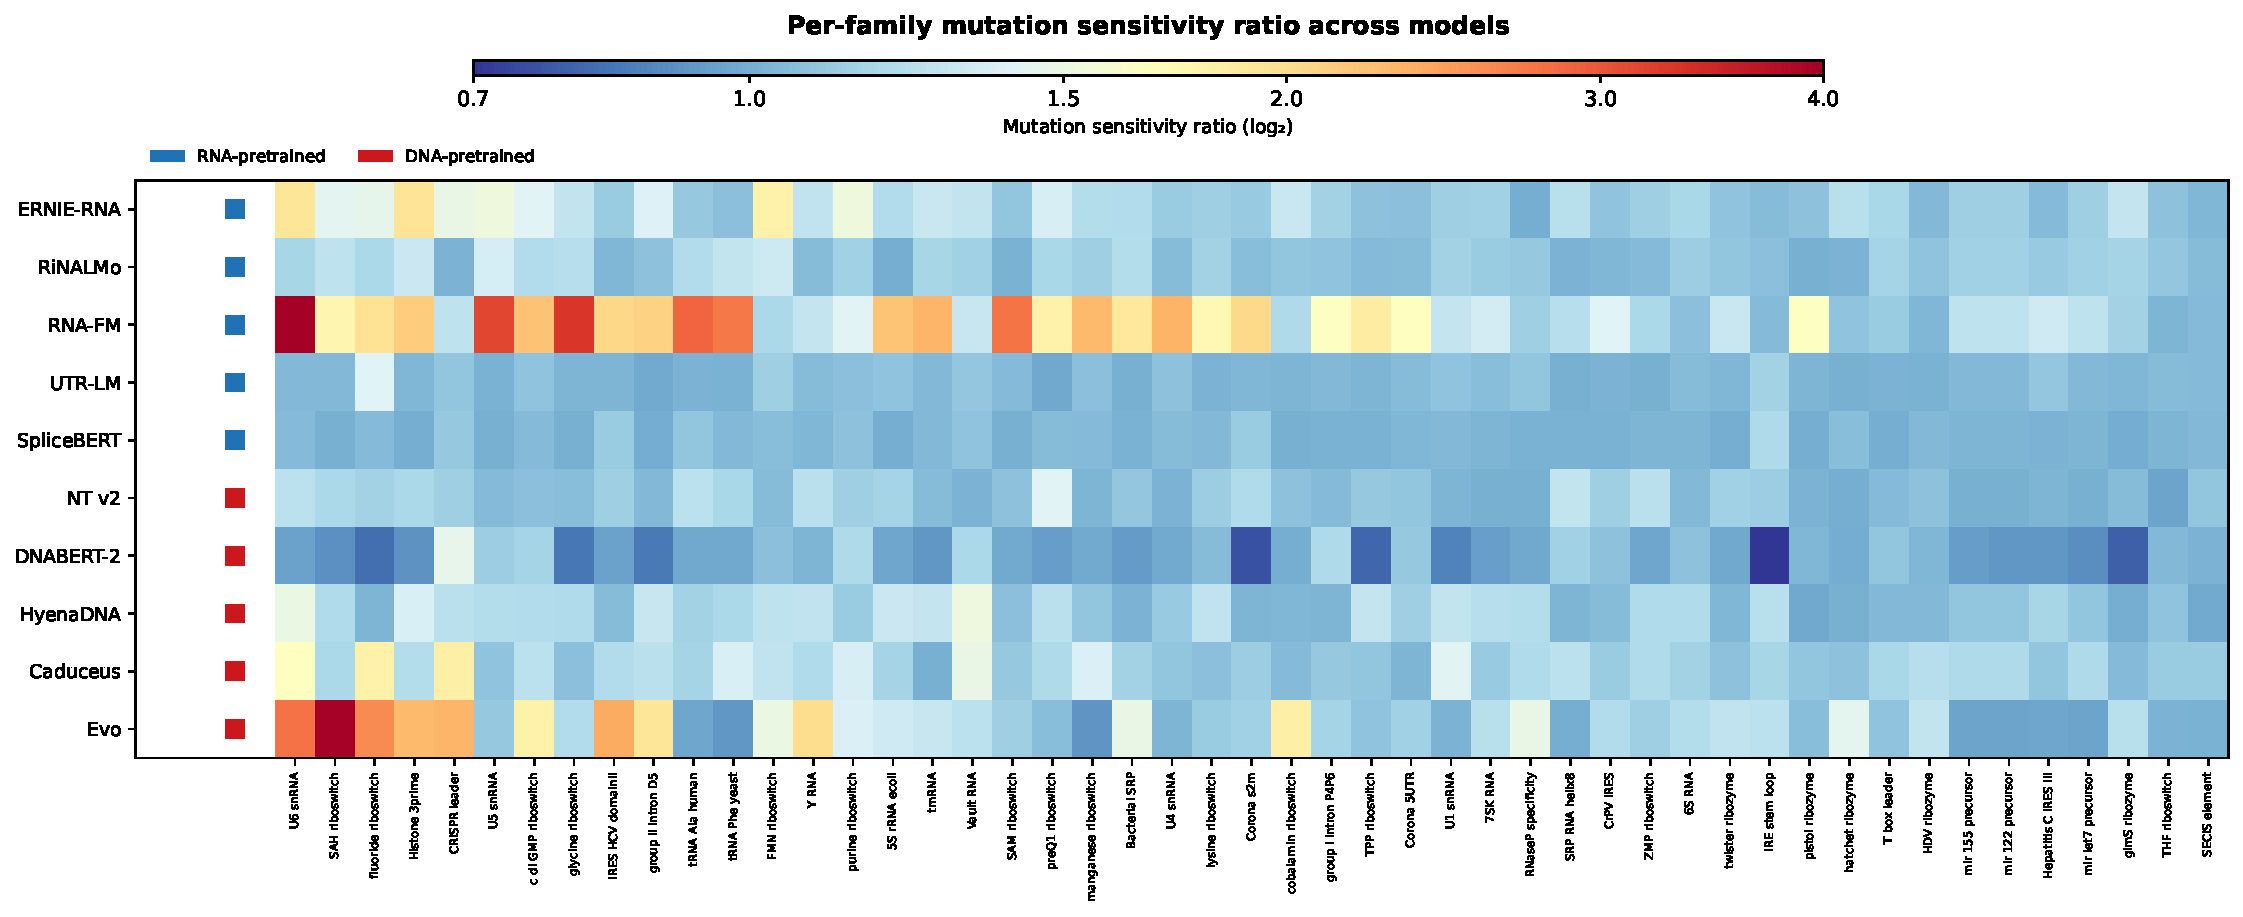
\includegraphics[width=\textwidth]{figures/fig_heatmap_wide.pdf}
\caption{Per-family mutation sensitivity ratio (log$_2$ scale) across
10 models and 49 Rfam families (sorted by mean ratio, descending).
ERNIE-RNA and RiNALMo show broad, moderate elevation across most
families; RNA-FM and Evo show high ratios in a few families but near-baseline
elsewhere. Blue/red squares indicate RNA/DNA pretraining.}
\label{fig:heatmap}
\end{figure}

\subsection{Rung 2: Dinucleotide controls separate genuine structure encoding}

\begin{table}[htbp]
\centering
\caption{Dinucleotide-stratified null results across all models.
``Fam $>$ nuc'' is the number of families exceeding the
nucleotide-stratified null; ``Survive dinuc'' is how many of those
also exceed the dinucleotide-stratified null. Bootstrap 95\% CIs
on retention rate computed by resampling families ($B = 10{,}000$).}
\label{tab:rung2}
\small
\begin{tabular}{lrrll}
\toprule
\textbf{Model} & \textbf{Fam $>$ nuc} & \textbf{Survive dinuc} & \textbf{Retention} & \textbf{95\% CI} \\
\midrule
ERNIE-RNA (86M, RNA)    & 31 & 30 & 97\% & [0.90, 1.00] \\
RiNALMo (650M, RNA)     & 18 & 16 & 89\% & [0.72, 1.00] \\
NT~v2 (56M, DNA)        & 14 & 11 & 79\% & [0.57, 1.00] \\
HyenaDNA (5.4M, DNA)    & 10 &  8 & 80\% & [0.50, 1.00] \\
Evo (7B, DNA)           & 10 &  7 & 70\% & [0.40, 1.00] \\
Caduceus (14M, DNA)     &  8 &  2 & 25\% & [0.00, 0.62] \\
DNABERT-2 (117M, DNA)   &  7 &  2 & 29\% & [0.00, 0.57] \\
SpliceBERT (19M, RNA)   &  4 &  2 & 50\% & [0.00, 1.00] \\
UTR-LM ($\sim$2M, RNA)  &  3 &  2 & 67\% & [0.00, 1.00] \\
RNA-FM (99M, RNA)       &  2 &  2 & 100\% & --- \\
\midrule
ERNIE-RNA untrained     &  3 &  1 & 33\% & [0.00, 1.00] \\
\bottomrule
\end{tabular}
\end{table}

The dinucleotide null produces a sharp separation between models.
ERNIE-RNA retains 30 of 31 first-order survivors (97\%): its
embedding-level structure signal persists after controlling for both
nucleotide and dinucleotide composition. RiNALMo retains 16 of 18
(89\%). Three DNA models---NT~v2 (11/14), HyenaDNA (8/10), and Evo
(7/10)---retain the majority of their families, suggesting
composition-independent structure encoding despite DNA-only
pretraining.

The remaining models collapse. Caduceus retains 2 of 8 (25\%),
DNABERT-2 retains 2 of 7 (29\%), and SpliceBERT retains 2 of 4.
ERNIE-RNA with randomized weights retains 1 of 3---consistent with
the architectural attention bias providing capacity without content.

The two-order cascade thus functions as a model-level discriminator
(Figure~\ref{fig:overview}):
models with genuine structure encoding largely survive the second
control, while those driven by composition lose most of their signal.

\begin{figure}[htbp]
\centering
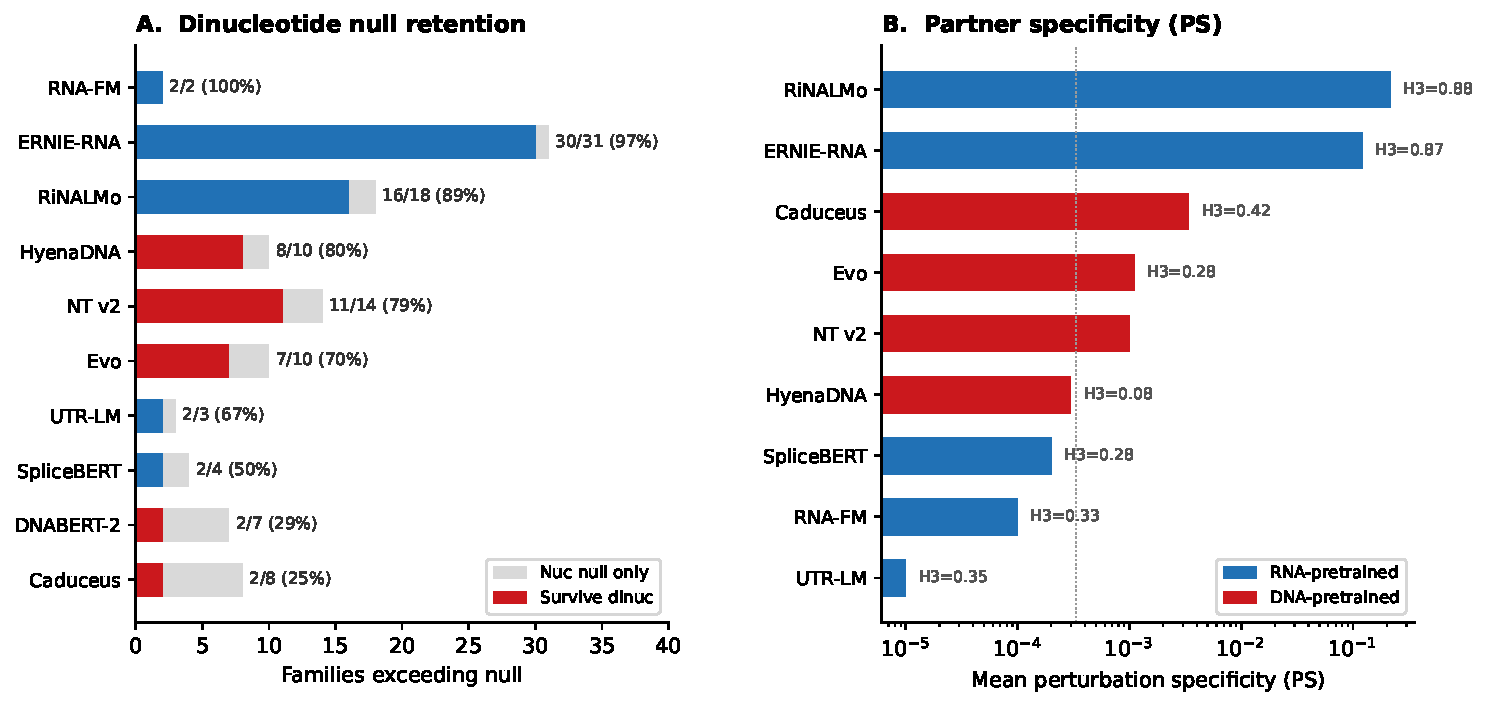
\includegraphics[width=\textwidth]{figures/fig_overview.pdf}
\caption{Summary of Rungs~2 and~3. \textbf{(A)}~Dinucleotide null
retention: grey bars show families exceeding the nucleotide-stratified
null; colored bars show how many survive the dinucleotide control.
ERNIE-RNA retains 30/31 (97\%), RiNALMo 16/18 (89\%).
\textbf{(B)}~Mean perturbation specificity (PS) on a log scale.
RiNALMo and ERNIE-RNA separate from the remaining models by two
orders of magnitude. H3 annotations show partner-is-max precision
(chance baseline $= 1/3$). DNABERT-2 omitted (negative PS).}
\label{fig:overview}
\end{figure}

\subsection{Rung 3: Two models know which base pairs with which}

This is the most demanding test, and it produces the clearest result.

\begin{table}[htbp]
\centering
\caption{Perturbation specificity across models. RiNALMo and
ERNIE-RNA separate from the pack by two orders of magnitude.
34 of 52 families qualify ($\geq 15$ WC pairs with $\geq 3$
per stem); NT~v2 and DNABERT-2 evaluate fewer due to tokenization.}
\label{tab:rung3}
\small
\begin{tabular}{llrccc}
\toprule
\textbf{Model} & \textbf{Domain} & \textbf{Mean PS} & \textbf{Gate} & \textbf{$>$ null} & \textbf{H3 prec.} \\
\midrule
\textbf{RiNALMo} (650M)    & RNA & \textbf{0.2150} & 31/34 & \textbf{30/31} & \textbf{0.882} \\
\textbf{ERNIE-RNA} (86M)  & RNA & \textbf{0.1204} & 31/34 & \textbf{29/31} & 0.874 \\
ERNIE-RNA untrained        & RNA & $9.5 \times 10^{-8}$ & 10/34 & 9/10 & --- \\
Caduceus (14M)             & DNA & 0.0034 & 16/34 & 13/16 & 0.416 \\
Evo (7B)                   & DNA & 0.0011 & 10/34 & 4/10 & 0.278 \\
SpliceBERT (19M)           & RNA & 0.0002 & 22/34 & 15/22 & 0.276 \\
HyenaDNA (5.4M)            & DNA & 0.0003 & 27/34 & 10/27 & 0.083 \\
RNA-FM (99M)               & RNA & 0.0001 & 8/34 & 4/8 & 0.325 \\
UTR-LM ($\sim$2M)          & RNA & 0.00001 & 16/34 & 13/16 & 0.350 \\
NT~v2 (56M)                & DNA & 0.001 & 1/4 & 0/1 & --- \\
DNABERT-2 (117M)           & DNA & $-0.016$ & 0/8 & --- & --- \\
\bottomrule
\end{tabular}
\end{table}

RiNALMo achieves the highest perturbation specificity (PS $= 0.215$),
with 30 of 31 gate-passing families exceeding the derangement null
and a partner-is-max precision of 0.882.
ERNIE-RNA follows at PS $= 0.120$, with 29/31 families exceeding the
null and H3 precision of 0.874. Both are two orders
of magnitude above the third model and far exceed the
$1/3$ chance baseline ($p \ll 0.001$, binomial test).

Caduceus (14M, DNA, BiMamba SSM) ranks third at PS $= 0.003$, with
13/16 gate-passing families exceeding the null and H3 precision of
0.416---above chance but two orders of magnitude below the leaders.
The remaining models cluster near zero PS. SpliceBERT
exceeds the null in 15 of 22 gate-passing families, but its PS
magnitude (0.0002) is three orders of magnitude below the two
leaders. HyenaDNA's H3 fraction (0.083) falls \emph{below} chance,
meaning it systematically perturbs partners less than adjacent
positions. The gap between the two leaders and the rest is
qualitative.

\paragraph{The untrained control confirms learning is necessary.}
ERNIE-RNA with randomized weights---preserving the architectural
attention bias but destroying all learned parameters---produces
$\text{PS} = 9.5 \times 10^{-8}$, six orders of magnitude below
the trained model. Only 10 of 34 families pass the positive control
gate (versus 31/34 trained). Of those 10 gate-passing families,
9 exceed the derangement null---a seemingly high rate that reflects
the gate's role as a filter: families that pass the gate with random
weights happen to have stem/loop distributions where even random
perturbations produce above-chance stem sensitivity, and the
derangement null within those selected families is correspondingly
easy to exceed. The absolute PS magnitude ($10^{-7}$) confirms that
no meaningful partner specificity is present. Architecture without
training produces nothing.

\paragraph{The attention bias is redundant after pretraining.}
ERNIE-RNA includes a pairwise attention bias that encodes
Watson-Crick pairing preferences. Zeroing this bias and running the
full Rung~1 pipeline yields a mean ratio of 1.235 (versus 1.242
trained), 32/49 families exceeding the nucleotide null (versus 31),
30/49 surviving the dinucleotide null (identical), attention contact
$\rho = 0.101$ (versus 0.100), and probing accuracy 0.666
(identical). The ablated model matches or marginally exceeds the trained model on
every metric. ERNIE-RNA's structure awareness resides entirely in learned
weights; the architectural bias provides capacity but is functionally
redundant given sufficient pretraining. This result---combined with the
untrained control showing that the bias alone produces nothing---indicates
that the bias accelerates or stabilizes learning of pairing patterns
during pretraining, but the learned representations carry the signal
at inference time.

\paragraph{Deep-layer concentration distinguishes real from spurious signal.}
RiNALMo's PS peaks at layer~33 (of 34) in 30 of 31 gate-passing
families. ERNIE-RNA peaks at layers~10--12 (of 12). The weak-signal
models peak at layers~0--1, consistent with tokenization and
positional-encoding artifacts.

\paragraph{Tokenization limits some evaluations.}
NT~v2's 6-mer tokenization makes single-nucleotide complement swaps
ambiguous (a swap at one position changes up to six overlapping
tokens); only 1 of 4 evaluable families passed the gate. DNABERT-2's
BPE tokenizer limits evaluation to 8 of 52 families; none pass. These
models' near-zero or negative PS reflects tokenization constraints as
much as architectural ones; their Rung~1 attention-contact signal
(above) shows they encode structure through a different channel.

\paragraph{Pretraining domain does not predict performance.}
The preregistered hypothesis H2$_6$ predicted that RNA-pretrained
models would outperform DNA-pretrained models on partner specificity.
This fails ($r_b = -0.28$, $p = 0.265$): Caduceus (14M, DNA) exceeds
three RNA models (SpliceBERT, RNA-FM, UTR-LM) on PS. The two leaders
happen to be RNA-pretrained, but pretraining domain alone does not
explain their success---ERNIE-RNA's bias accelerates learning at
smaller scale (86M) and RiNALMo's 650M parameters reach the same
capability without it.

\subsection{Case study: Huntington's disease repeat-expansion alleles}

The composition confound has direct clinical consequences. CAG
trinucleotide repeats in HTT exon~1 have identical nucleotide
composition regardless of repeat count, yet ViennaRNA
MFE~\citep{vienna2011} confirms that they form progressively larger
stem-loop structures ($-24.8$~kcal/mol at CAG10 to
$-112.3$~kcal/mol at CAG80). A composition-sensitive model will
produce identical predictions for structurally distinct alleles.

\begin{table}[htbp]
\centering
\caption{Embedding cosine distance from wild-type (CAG17). RNA-FM
produces near-identical embeddings for all allele lengths; ERNIE-RNA
shows monotonic increase with repeat count.}
\label{tab:htt}
\small
\begin{tabular}{lcccc}
\toprule
\textbf{Model} & \textbf{CAG21} & \textbf{CAG36} & \textbf{CAG40} & \textbf{CAG60} \\
\midrule
ERNIE-RNA & $5.8 \times 10^{-4}$ & $7.2 \times 10^{-3}$ & $9.1 \times 10^{-3}$ & $\mathbf{2.3 \times 10^{-2}}$ \\
RNA-FM    & 0.0 & 0.0 & $3.6 \times 10^{-7}$ & $3.0 \times 10^{-7}$ \\
\bottomrule
\end{tabular}
\end{table}

We tested ERNIE-RNA and RNA-FM on four clinically relevant allele
lengths (CAG21, CAG36, CAG40, CAG60) with CAG17 (normal) as baseline
(Table~\ref{tab:htt}). RNA-FM produces near-identical embeddings
across all lengths (cosine distance $< 10^{-6}$), confirming the
composition confound in a clinical context. ERNIE-RNA shows monotonic
increase with repeat length, reaching $0.023$ between CAG17 and
CAG60---four orders of magnitude above RNA-FM. This comparison is
clean because it holds composition constant and varies only structure,
applying the Rung~2 principle to allele-selective antisense
oligonucleotide design.

\subsection{Preregistered hypothesis summary}

\begin{table}[htbp]
\centering
\caption{Preregistered hypothesis results.}
\label{tab:hypotheses}
\small
\begin{tabular}{llll}
\toprule
\textbf{Hyp.} & \textbf{Criterion} & \textbf{Result} & \textbf{Verdict} \\
\midrule
H1    & RNA-FM ratio $\geq 2.0$ ($N$=12) & 1.74$\times$ & FAIL \\
H6    & RNA-FM ratio $\geq 2.0$ ($N$=52) & 1.75$\times$ & FAIL \\
H7    & $\geq 1$ family survives dinuc null & 30 fam (ERNIE-RNA) & \textbf{PASS} \\
H10   & RNA-FM trained $>$ untrained $\geq 75$\% & 48/49 = 98\% & \textbf{PASS} \\
H11   & NT~v2 attn $> 0.15$ / $< 0.05$ untrained & 0.322 / 0.328 & FAIL$^\ddagger$ \\
\midrule
H1$_6$ & $\geq 1$ model: PS $> 0$, $\geq 7$ fam $>$ null & RiNALMo: 30/31; ERNIE-RNA: 29/31 & \textbf{PASS} \\
H2$_6$ & RNA PS $>$ DNA PS (rb $> 0.5$) & rb $= -0.28$, $p = 0.265$ & FAIL \\
H3$_6$ & Partner-is-max $> 1/3$ & RiNALMo: 0.882; ERNIE-RNA: 0.874 & \textbf{PASS} \\
\bottomrule
\end{tabular}

\smallskip\noindent{\footnotesize $^\ddagger$H11 originally passed
under the SDPA attention backend, which returned $\rho = 0.000$ for
untrained NT~v2. Corrected with eager attention: untrained
$\rho = 0.328$ (see Table~\ref{tab:attn_trained_untrained}).
H2$_6$ includes all 10 models
($n_{\text{RNA}} = 5$, $n_{\text{DNA}} = 5$). Caduceus (DNA) achieves
higher PS than three RNA models, reversing the effect direction.}
\end{table}


%% ======================================================================
\section{Discussion}
%% ======================================================================

\subsection{What the two leaders do differently}

ERNIE-RNA and RiNALMo achieve partner specificity through distinct
mechanisms. ERNIE-RNA (86M) includes a pairwise attention bias that
steers attention toward Watson-Crick and wobble pairs from the
second transformer layer onward~\citep{ernierna2025}. Zeroing this
bias at inference time leaves every Rung~1 metric unchanged (mean
ratio 1.235 vs 1.242; dinucleotide retention 30/49 in both
conditions; probing accuracy 0.666 in both). The bias is functionally
redundant after pretraining: learned weights carry the entire
structural signal. Combined with the untrained control showing the
bias alone produces nothing, this indicates that the bias accelerates
learning during pretraining but is absorbed into learned
representations by convergence.

RiNALMo (650M) uses standard attention with no structural bias.
Three other RNA models (RNA-FM, SpliceBERT, UTR-LM) also use standard
MLM on RNA without structural bias and produce negligible PS. The
difference is scale: RiNALMo's 650M parameters cross a threshold at
which MLM on RNA sequences can learn partner specificity without
architectural assistance.

Both models concentrate PS in the final layers: ERNIE-RNA at
layers~10--12 (of 12), RiNALMo at layer~33 (of 34). The weak-signal
models peak at layers~0--1. Deep-layer concentration distinguishes
learned pairing from tokenization artifacts.

Caduceus (14M, BiMamba SSM, DNA) ranks third by PS magnitude (0.003),
with 13/16 gate-passing families exceeding the derangement null and
H3 precision of 0.416---above the $1/3$ chance level. This places a
DNA SSM above three RNA attention models. We hypothesize that Caduceus's bidirectional
architecture, which processes the sequence in both directions
simultaneously, gives it access to long-range dependencies that
unidirectional SSMs (HyenaDNA, Evo) lack---a plausible advantage for
detecting base-pairing, which is inherently bidirectional. This
hypothesis is consistent with the observation but untested; a
controlled comparison with a unidirectional Mamba variant trained on
the same data would be needed to confirm directionality as the causal
factor. The failure of H2$_6$ (RNA-pretrained PS $>$ DNA-pretrained
PS) is itself informative. Caduceus, a 14M-parameter DNA model,
achieves higher PS than three RNA models with 5--50$\times$ more
parameters. Bidirectional processing may be more predictive of
pairing detection than RNA-specific pretraining at smaller scales.

The attention channel provides an independent read on structure
knowledge, but with an important caveat. NT~v2 produces the highest
attention-contact correlation ($\rho = 0.322$), yet this signal is
entirely architectural: untrained NT~v2 produces $\rho = 0.328$,
and the per-family delta averages $-0.006$ with no systematic
direction (Table~\ref{tab:attn_trained_untrained}). NT~v2's 6-mer
tokenization aggregates base-pairing partners into adjacent tokens,
producing structured attention from positional proximity alone.
DNABERT-2's content-only attention ($\rho = 0.257$ trained vs $0.000$
untrained) is the sole model showing learned attention-contact
structure; the practical attention including ALiBi position biases
would produce a lower correlation, so $0.257$ is an upper bound.
Among the five character-tokenized RNA models, all show trained
attention within $\pm 0.025$ of untrained---no model learns
attention-level structure beyond what its architecture provides.
Attention-contact correlation and embedding-level PS are qualitatively
different: the former measures a statistical association that can
arise from tokenization or positional encoding, while PS is a causal
test requiring the model to encode specific pairing relationships.

\subsection{Upper bound on non-covariation signal}

ERNIE-RNA's partner specificity could reflect sequence covariation
rather than learned geometric pairing. Compensatory mutations that
maintain base pairing are overrepresented in evolutionary RNA
alignments; a model trained on such sequences might predict that
mutating one position perturbs its covarying partner without encoding
the physical mechanism of pairing.

To estimate the covariation contribution, we generated synthetic
sequences for each Rfam family: the dot-bracket structure is
preserved exactly, but nucleotides are assigned randomly (uniform
Watson-Crick pairs at paired positions, uniform random at unpaired).
These sequences share structure with their natural counterparts but
carry no evolutionary covariation. Importantly, this ablation also
destroys sequence context and positional composition gradients
present in natural RNA, so the residual PS on synthetic sequences
represents an upper bound on the non-covariation contribution---it
includes any signal from base-pairing geometry that survives context
destruction, but cannot isolate covariation from these other signals.

ERNIE-RNA's mean PS drops from 0.120 (natural) to 0.035 (synthetic),
a 71\% reduction. RiNALMo drops from 0.215 to 0.061, a 71\%
reduction. Both models lose roughly 70\% of their PS when covariation
and sequence context are jointly removed. The residual synthetic
PS---still orders of magnitude above the weak-signal
models---indicates that some fraction of partner specificity
derives from structural features beyond covariation, though this
experiment cannot determine the exact decomposition.

\paragraph{MI baseline.}
As an independent check, we computed mutual information (MI) between
paired positions from Rfam seed alignments (51 families, $n \geq 3$
sequences each). MI cleanly separates paired from unpaired positions
(mean MI $= 0.349$ vs $0.063$; Wilcoxon $p = 3.5 \times 10^{-10}$),
confirming that evolutionary covariation is detectable in the
alignments. Per-family mean MI shows a weak positive trend with
model PS that does not reach significance at this sample size
(ERNIE-RNA: $\rho = 0.320$, $p = 0.065$; RiNALMo:
$\rho = 0.265$, $p = 0.130$; $N = 51$ families). With 51
observations, the analysis is underpowered to detect moderate
correlations ($\rho < 0.3$); a larger family panel would be
needed to resolve whether high-covariation families produce
systematically higher PS.

\subsection{Limitations}
\label{sec:limitations}

\paragraph{Single representative per family.}
Each family is represented by a single seed sequence selected by
highest bit score. To quantify within-family variance, we ran
ERNIE-RNA and RiNALMo on 3--5 alternative Rfam seed sequences for
each of 51 families (253 sequences total). The mean coefficient of
variation (CV) of the mutation sensitivity ratio across sequences
within a family is 0.057 (median 0.055) for ERNIE-RNA and 0.037
(median 0.032) for RiNALMo. Both models show within-family
sequence choice contributing less than 6\% noise, well below the
preregistered threshold of 10\%. The consistency across two models
with different architectures (ERNIE-RNA: transformer encoder;
RiNALMo: large RNA language model) and tokenization strategies
suggests the single-sequence design introduces minimal variance.
The bootstrap 95\% CIs reported in
Tables~\ref{tab:rung1}--\ref{tab:rung2} resample over families and
capture between-family variance; they do not directly account for
within-family sequence choice, though the $\leq$6\% CV observed
for both models suggests this component is small relative to
between-family differences.

\paragraph{Structure representation.}
The evaluation uses Rfam consensus secondary structures (dot-bracket
notation), which cannot represent pseudoknots, kissing loops, or
other non-nested base pairings. Of the 52 families in our panel,
approximately 12 (23\%) have known pseudoknots or non-canonical
tertiary interactions documented in their Rfam or PDB annotations.
For these families, some base-paired positions are labeled as
``unpaired'' in dot-bracket notation, introducing systematic label
noise. Structure awareness as measured here is therefore limited to
nested secondary structure, and models that encode pseudoknot
interactions may receive less credit than they deserve at Rungs~1--2.

\paragraph{Multiple testing.}
Each family is tested independently against its own permutation null
at $\alpha = 0.05$. With 49 families, 2.45 are expected to exceed the
null by chance under independence. A binomial test on
the number of exceedances provides a global assessment: under the
null of independent $\alpha = 0.05$ tests, observing $\geq 31$ of 49
(ERNIE-RNA) has $p < 10^{-20}$; $\geq 18$ of 49 (RiNALMo) has
$p < 10^{-10}$. Models with 2--4 exceedances (UTR-LM at 3, SpliceBERT
at 4, RNA-FM at 2, ERNIE-RNA untrained at 3) are
indistinguishable from the false-positive floor ($p > 0.3$,
binomial). Applying Benjamini-Hochberg correction at FDR $= 0.05$
within each model reduces the counts modestly for top models
(ERNIE-RNA: 31 $\to$ 28; RiNALMo: 18 $\to$ 15) and
zeros out floor-level models entirely. The main text reports
uncorrected per-family counts because the permutation null already
controls the per-test type~I error rate, but the BH-adjusted counts
confirm that the separation between the top two models and the rest
survives correction.

\paragraph{No held-out validation set.}
The metric definitions, gate thresholds, and layer-selection strategy
were developed on the same 52 families used for evaluation. A
held-out family split would strengthen the claim that the framework
generalizes to unseen RNA structures. The permutation nulls are
computed per family and do not overfit to the evaluation set in the
classical sense---the null distribution is regenerated for each
family independently. The model-level exceedance counts, however,
are aggregate statistics that could in principle be inflated if the
family selection were biased toward families where the method
performs well. We note that the families were selected by structural
diversity criteria (spanning 8 major ncRNA classes) with no reference
to model performance, and the per-family heatmap
(Figure~\ref{fig:heatmap}) shows broad coverage rather than outlier-driven
results. A held-out replication on an independent family sample is a
priority for future validation.

\paragraph{Best-layer selection.}
The mutation sensitivity ratio selects the best layer per family by
$\max_\ell R^{(\ell)}$, which inflates the test statistic. The
permutation null mirrors this optimization---each permuted replicate
also takes $\max_\ell$---so the comparison is fair within each family.
The inflation affects the magnitude of reported ratios but does not
affect the exceedance decision.

\paragraph{Tokenization and Rung~3.}
NT~v2 and DNABERT-2 tokenization constraints limit the Rung~3
evaluation. These models' near-zero PS results reflect the limits of
single-nucleotide evaluation on multi-nucleotide tokenizers; their
attention-contact correlation provides the relevant structural signal
for these architectures.

\paragraph{Probing margins and the PS--probing disconnect.}
ERNIE-RNA shows the strongest probing margin above chance
($\Delta = +0.166$, balanced accuracy $= 0.666$ at layer~11),
followed by RiNALMo ($\Delta = +0.123$ at layer~32). The remaining
models cluster between $+0.031$ and $+0.077$. These margins are
modest even for the leaders, despite their strong PS. The disconnect
reflects a difference in what each metric tests. The linear probe
classifies single-position representations as stem or loop, a task
that composition-matched nucleotides make difficult by design.
Probing classifiers are known to be weak instruments for detecting
relational knowledge~\citep{belinkov2022probing,hewitt2019control}:
a model can encode structure in cross-position interaction patterns
that a per-position linear probe cannot access. PS avoids this
limitation as a causal perturbation test that directly measures
relational knowledge (whether mutating position $i$ selectively
perturbs position $j$).

\subsection{Practical implications}

For downstream applications---antisense oligonucleotide design,
splice-site prediction, RNA design---the results carry a direct
consequence. RiNALMo and ERNIE-RNA encode genuine pairing topology
and could support structure-dependent predictions. The remaining eight
models should be paired with physics-based tools such as
ViennaRNA~\citep{vienna2011} for any application requiring resolution
beyond stem-versus-loop discrimination.

The composition null provides a practical quality gate: it certifies
whether a model's structural predictions reflect learned pairing or
nucleotide composition. For repeat-expansion therapeutic targets,
where composition is uniform across alleles, models failing this gate
will produce identical predictions for structurally distinct alleles.


%% ======================================================================
\section{Conclusion}
%% ======================================================================

RNA structure awareness in foundation models is rarer and more
specific than naive metrics suggest. Composition controls separate
models into two tiers: ERNIE-RNA and RiNALMo retain the vast majority
of their families through dinucleotide stratification (30/31 and
16/18), while eight models retain at most two each. The hardest
test---partner specificity with a derangement null---produces the
clearest result: two of ten models encode which specific position
pairs with which (RiNALMo, $\text{PS} = 0.215$, 88.2\% precision;
ERNIE-RNA, $\text{PS} = 0.120$, 87.4\% precision). RiNALMo achieves
this through scale on RNA data; ERNIE-RNA through an architectural
base-pairing bias. The remaining eight models are indistinguishable
from the null. The three-rung framework provides a reusable template
for evaluating structure awareness in sequence foundation models.


\section*{Availability and Implementation}

The evaluation framework is implemented in Python using PyTorch,
Hugging Face Transformers, and the multimolecule library. All analysis
scripts, per-family result files, 52 Rfam structures, and
preregistration documents (SHAs listed in Section~3.1) are available at
\url{https://github.com/elliottower/rna-structure-awareness} and
deposited on Zenodo (DOI:
\href{https://doi.org/10.5281/zenodo.21362717}{10.5281/zenodo.21362717})
under a CC-BY-4.0 license.

\section*{Declarations}

\paragraph{Ethics approval and consent to participate.}
This study uses exclusively publicly available pretrained model weights
and published RNA sequences. No human subjects or animal subjects were
involved. No ethical approval was required.

\paragraph{Competing interests.}
The author declares no competing interests.

\paragraph{Funding.}
None. This work was conducted independently.

\paragraph{Authors' contributions.}
E.T.: Conceptualization, Methodology, Software, Formal analysis,
Investigation, Data curation, Writing -- original draft, Writing --
review \& editing, Visualization.

\paragraph{Acknowledgements.}
The author used Claude Code~\citep{claudecode} to assist with drafting
and editing manuscript text and with writing and debugging analysis code.
The author reviewed and verified all outputs, takes full responsibility
for the accuracy and integrity of the work, and confirms that all
hypotheses, preregistered predictions, interpretations, and conclusions
are the author's own.


%% ======================================================================
\begin{thebibliography}{99}

\bibitem[Chen et~al., 2022]{rnafm2022}
Chen, J., Hu, Z., Sun, S., et~al. (2022).
Interpretable RNA Foundation Model from Unannotated Data for Highly
Accurate RNA Structure and Function Predictions.
\emph{Nature Methods}, 19, 1616--1621.

\bibitem[Yin et~al., 2025]{ernierna2025}
Yin, W., Zhang, Z., Zhang, S., et~al. (2025).
ERNIE-RNA: An RNA Language Model with Structure-Enhanced Representations.
\emph{Nature Communications}, 16, 10076.

\bibitem[Peni\'c et~al., 2025]{rinalmo2025}
Peni\'c, R.J., Vla\v{s}i\'c, T., Huber, R.G., Wan, Y.,
\v{S}iki\'c, M. (2025).
RiNALMo: General-Purpose RNA Language Models Can Generalize Well on
Structure Prediction Tasks.
\emph{Nature Communications}, 16, 5729.

\bibitem[Chu et~al., 2024]{utrlm2024}
Chu, Y., Yu, D., Li, Y., et~al. (2024).
A 5$'$ UTR Language Model for Decoding Untranslated Regions of mRNA and
Function Predictions.
\emph{Nature Machine Intelligence}, 6, 449--460.

\bibitem[Chen et~al., 2024]{splicebert2024}
Chen, K., Zhou, Y., Ding, M., Wang, Y., Ren, Z., Yang, Y. (2024).
Self-supervised learning on millions of primary RNA sequences improves
sequence-based RNA splicing prediction.
\emph{Briefings in Bioinformatics}, 25(3), bbae163.

\bibitem[Dalla-Torre et~al., 2024]{ntv22024}
Dalla-Torre, H., Gonzalez, L., Mendoza-Revilla, J., et~al. (2024).
The Nucleotide Transformer: Building and Evaluating Robust Foundation
Models for Human Genomics.
\emph{Nature Methods}, 21, 1176--1181.

\bibitem[Zhou et~al., 2024]{dnabert22024}
Zhou, Z., Ji, Y., Li, W., Dutta, P., Davuluri, R., Liu, H. (2024).
DNABERT-2: Efficient Foundation Model and Benchmark for Multi-Species
Genomes. ICLR 2024. arXiv:2306.15006.

\bibitem[Nguyen et~al., 2023]{hyenadna2023}
Nguyen, E., Poli, M., Faber, M., et~al. (2023).
HyenaDNA: Long-Range Genomic Sequence Modeling at Single Nucleotide
Resolution.
\emph{Advances in Neural Information Processing Systems} (NeurIPS 2023).

\bibitem[Schiff et~al., 2024]{caduceus2024}
Schiff, Y., Kao, C.-H., Gokaslan, A., et~al. (2024).
Caduceus: Bi-Directional Equivariant Long-Range DNA Sequence Modeling.
\emph{Proceedings of the 41st International Conference on Machine
Learning} (ICML 2024).

\bibitem[Nguyen et~al., 2024]{evo2024}
Nguyen, E., Poli, M., Durrant, M.G., et~al. (2024).
Sequence Modeling and Design from Molecular to Genome Scale with Evo.
\emph{Science}, 386(6723).

\bibitem[Kalvari et~al., 2021]{rfam2021}
Kalvari, I., Nawrocki, E.P., Ontiveros-Palacios, N., et~al. (2021).
Rfam 14: expanded coverage of metagenomic, viral and microRNA families.
\emph{Nucleic Acids Research}, 49(D1), D192--D200.

\bibitem[Lorenz et~al., 2011]{vienna2011}
Lorenz, R., Bernhart, S.H., Höner zu Siederdissen, C., et~al. (2011).
ViennaRNA Package 2.0.
\emph{Algorithms for Molecular Biology}, 6, 26.

\bibitem[Belinkov, 2022]{belinkov2022probing}
Belinkov, Y. (2022).
Probing Classifiers: Promises, Shortcomings, and Advances.
\emph{Computational Linguistics}, 48(1), 207--219.

\bibitem[Hewitt \& Liang, 2019]{hewitt2019control}
Hewitt, J. \& Liang, P. (2019).
Designing and Interpreting Probes with Control Tasks.
\emph{Proceedings of EMNLP 2019}, 2733--2743.

\bibitem[Anthropic, 2025]{claudecode}
Anthropic. (2025).
Claude Code. \url{https://claude.ai/code}.

\end{thebibliography}

\end{document}
